\documentclass[11pt,a4paper,oneside]{report}
% Attend — Shared LaTeX preamble
\usepackage[utf8]{inputenc}
\usepackage[T1]{fontenc}
\usepackage{lmodern}
\usepackage[margin=1in, headheight=15pt]{geometry}
\usepackage{graphicx}
\usepackage{xcolor}
\usepackage{booktabs}
\usepackage{longtable}
\usepackage{array}
\usepackage{enumitem}
\usepackage{listings}
\usepackage{hyperref}
\usepackage{fancyhdr}
\usepackage{titlesec}
\usepackage{tikz}
\usepackage{float}
\usepackage{caption}
\usepackage{microtype}
\usepackage{amsmath}
\usepackage{amssymb}

\usetikzlibrary{arrows.meta, positioning, shapes.geometric, fit, calc, shadows}

\definecolor{AttendPrimary}{HTML}{1E3A5F}
\definecolor{AttendAccent}{HTML}{2563EB}
\definecolor{AttendLight}{HTML}{EFF6FF}
\definecolor{AttendGray}{HTML}{64748B}
\definecolor{AttendCodeBg}{HTML}{F8FAFC}
\definecolor{AttendBorder}{HTML}{CBD5E1}

\hypersetup{
  colorlinks=true,
  linkcolor=AttendPrimary,
  urlcolor=AttendAccent,
  pdftitle={Attend Section Management},
  pdfauthor={Attend Engineering Team}
}

\titleformat{\chapter}[display]
  {\normalfont\huge\bfseries\color{AttendPrimary}}
  {\chaptertitlename\ \thechapter}{16pt}{\Huge}
\titleformat{\section}
  {\normalfont\Large\bfseries\color{AttendPrimary}}{\thesection}{1em}{}
\titleformat{\subsection}
  {\normalfont\large\bfseries\color{AttendPrimary}}{\thesubsection}{1em}{}

\pagestyle{fancy}
\fancyhf{}
\fancyhead[L]{\small\textcolor{AttendGray}{Attend — Section Management}}
\fancyhead[R]{\small\textcolor{AttendGray}{v1.0}}
\fancyfoot[C]{\thepage}
\renewcommand{\headrulewidth}{0.4pt}

\lstdefinestyle{attendcode}{
  backgroundcolor=\color{AttendCodeBg},
  basicstyle=\ttfamily\small,
  keywordstyle=\color{AttendAccent}\bfseries,
  commentstyle=\color{AttendGray}\itshape,
  breaklines=true,
  frame=single,
  rulecolor=\color{AttendBorder},
  numbers=left,
  numberstyle=\tiny\color{AttendGray},
  tabsize=2,
  showstringspaces=false,
  captionpos=b
}
\lstset{style=attendcode}

\newcommand{\docversion}{1.0}
\newcommand{\docdate}{August 2026}


\begin{document}

% ===================== TITLE PAGE =====================
\begin{titlepage}
  \begin{tikzpicture}[remember picture, overlay]
    \fill[AttendPrimary] (current page.north west) rectangle ([yshift=-4.2cm]current page.north east);
    \node[anchor=west, text=white] at ([xshift=1.2cm, yshift=-2cm]current page.north west) {
      \begin{minipage}{0.85\textwidth}
        {\fontsize{32}{36}\selectfont\bfseries Attend}\\[0.35cm]
        {\fontsize{16}{20}\selectfont Section Management}\\[0.2cm]
        {\fontsize{11}{14}\selectfont Detailed Technical Reference}
      \end{minipage}
    };
    \fill[AttendLight] ([yshift=-4.2cm]current page.north west) rectangle (current page.south east);
  \end{tikzpicture}

  \vspace*{5cm}
  \begin{center}
    {\LARGE\bfseries\color{AttendPrimary} Section Management Module\\[0.15cm]
    Complete Specification\par}
    \vspace{1.5cm}
    \begin{tabular}{@{}ll@{}}
      \textbf{Document Version} & \docversion \\
      \textbf{Publication Date} & \docdate \\
      \textbf{Product} & Attend v1.0.0 \\
      \textbf{Scope} & Sections, teachers, students, attendance scoping \\
    \end{tabular}
    \vfill
    {\small\color{AttendGray}
      Covers data model, business rules, REST API, RBAC, mobile workflows,\\
      database triggers, and integration with face-recognition attendance.
    \par}
  \end{center}
\end{titlepage}

\tableofcontents
\listoffigures
\listoftables
\clearpage

% ===================== CHAPTER 1 =====================
\chapter{Overview}
\label{ch:overview}

\section{Purpose}

Section management is the organizational layer in Attend that subdivides a \textbf{subject} into teaching groups (e.g., Section A, Section B). Each section has its own teacher assignments and student roster. Attendance capture and face recognition are scoped to these rosters so that teachers only mark present the students they actually teach.

Without sections, recognition would match against all enrolled students in a college or subject, leading to incorrect attendance in multi-batch courses.

\section{Problem Statement}

In colleges, a single subject (e.g., ``Operating Systems'') is often taught to multiple batches:
\begin{itemize}[leftmargin=1.5em]
  \item Different time slots or classrooms
  \item Different faculty members
  \item Different student groups
\end{itemize}

Attend models this by allowing department administrators to create sections under a subject, assign teachers, and let teachers (or admins) build section rosters. Attendance sessions require an explicit \texttt{section\_id}, ensuring biometric matches are filtered to that section only.

\section{Core Business Rule}

\begin{center}
  \fbox{\parbox{0.92\textwidth}{
    \centering\bfseries
    A student may belong to at most \emph{one} section per subject.\\
    They cannot simultaneously be in Section A and Section B for the same subject.
  }}
\end{center}

This rule is enforced at the API layer \emph{and} by a PostgreSQL trigger (migration \texttt{002}).

\section{Entity Hierarchy}

\begin{figure}[H]
  \centering
  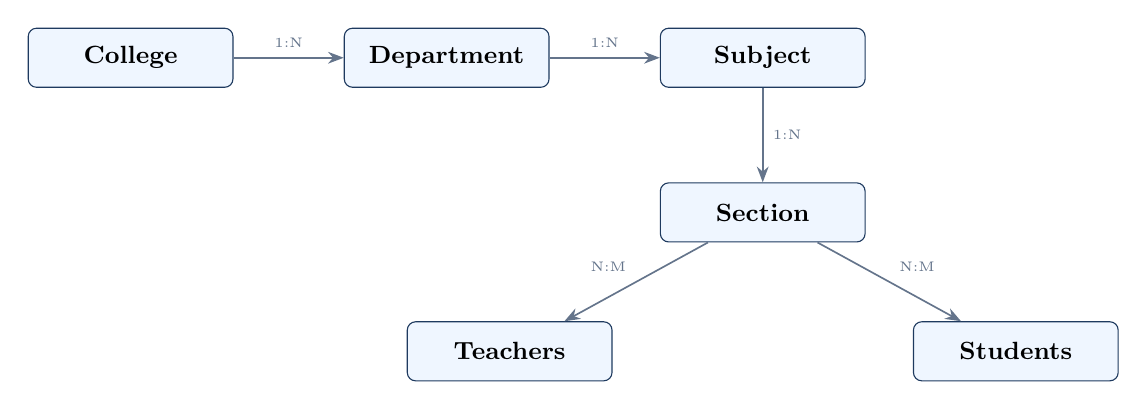
\begin{tikzpicture}[
    ent/.style={
      rectangle, rounded corners=3pt, draw=AttendPrimary, fill=AttendLight,
      minimum width=2.6cm, minimum height=0.75cm, align=center, font=\small\bfseries
    },
    arr/.style={-{Stealth[length=2mm]}, line width=0.6pt, color=AttendGray}
  ]
    \node[ent] (col) {College};
    \node[ent, right=1.4cm of col] (dep) {Department};
    \node[ent, right=1.4cm of dep] (sub) {Subject};
    \node[ent, below=1.2cm of sub] (sec) {Section};
    \node[ent, below left=1cm and 0.6cm of sec] (tea) {Teachers};
    \node[ent, below right=1cm and 0.6cm of sec] (stu) {Students};

    \draw[arr] (col) -- node[above, font=\tiny]{1:N} (dep);
    \draw[arr] (dep) -- node[above, font=\tiny]{1:N} (sub);
    \draw[arr] (sub) -- node[right, font=\tiny]{1:N} (sec);
    \draw[arr] (sec) -- node[above left, font=\tiny]{N:M} (tea);
    \draw[arr] (sec) -- node[above right, font=\tiny]{N:M} (stu);
  \end{tikzpicture}
  \caption{%
    \textbf{Section placement in the institutional hierarchy.}%
    Sections belong to exactly one subject. Teachers and students are linked to sections through junction tables. A student enrolled in Section A of Subject X cannot also appear in Section B of the same subject.
  }
  \label{fig:hierarchy}
\end{figure}

% ===================== CHAPTER 2 =====================
\chapter{Data Model}
\label{ch:data-model}

\section{Database Tables}

Section management introduces three primary tables (migration \texttt{001\_add\_sections.sql}) and extends the attendance table.

\begin{table}[H]
  \centering
  \caption{Section-Related Database Tables}
  \label{tab:tables}
  \begin{tabular}{@{}p{3.2cm}p{4.5cm}p{5.3cm}@{}}
    \toprule
    \textbf{Table} & \textbf{Key Columns} & \textbf{Purpose} \\
    \midrule
    \texttt{sections} & \texttt{id}, \texttt{subject\_id}, \texttt{name} & Named batch under a subject \\
    \texttt{section\_teachers} & \texttt{section\_id}, \texttt{teacher\_id} & Teacher--section assignment \\
    \texttt{section\_students} & \texttt{section\_id}, \texttt{student\_id} & Student--section enrollment \\
    \texttt{attendance} & \texttt{section\_id} (added) & Links attendance to a section \\
    \bottomrule
  \end{tabular}
\end{table}

\section{Constraints and Indexes}

\begin{itemize}[leftmargin=1.5em]
  \item \textbf{Unique section name:} \texttt{UNIQUE(subject\_id, name)} --- no duplicate ``A'' for the same subject.
  \item \textbf{Cascade delete:} Deleting a section removes its \texttt{section\_teachers} and \texttt{section\_students} rows.
  \item \textbf{Indexes:} On \texttt{sections.subject\_id}, \texttt{section\_teachers.teacher\_id}, \texttt{section\_students.student\_id}, \texttt{attendance.section\_id}.
  \item \textbf{Row Level Security (RLS):} Enabled on all three section tables with policies scoped to department/college membership.
\end{itemize}

\section{Entity Relationship Diagram}

\begin{figure}[H]
  \centering
  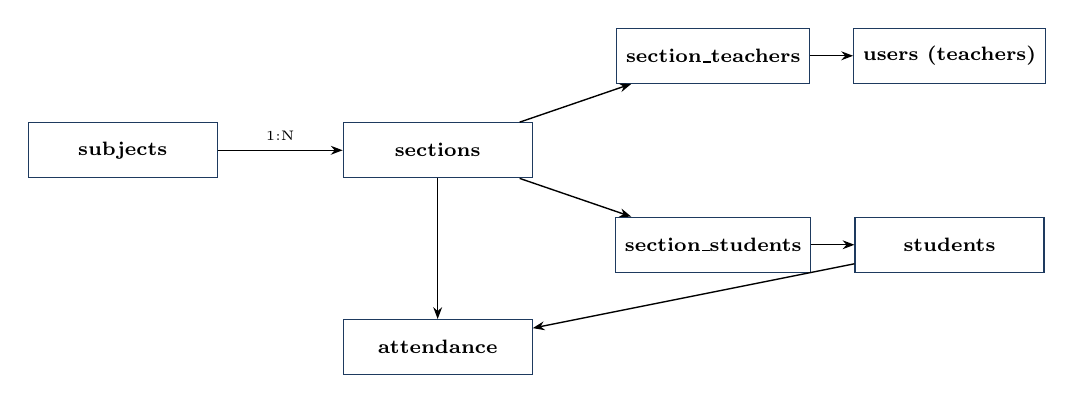
\begin{tikzpicture}[
    entity/.style={
      rectangle, draw=AttendPrimary, fill=white, minimum width=2.4cm,
      minimum height=0.7cm, align=center, font=\scriptsize\bfseries
    },
    rel/.style={-{Stealth[length=1.5mm]}, line width=0.5pt}
  ]
    \node[entity] (subjects) at (0,0) {subjects};
    \node[entity] (sections) at (4,0) {sections};
    \node[entity] (st) at (7.5,1.2) {section\_teachers};
    \node[entity] (ss) at (7.5,-1.2) {section\_students};
    \node[entity] (users) at (10.5,1.2) {users (teachers)};
    \node[entity] (students) at (10.5,-1.2) {students};
    \node[entity] (att) at (4,-2.5) {attendance};

    \draw[rel] (subjects) -- node[above, font=\tiny]{1:N} (sections);
    \draw[rel] (sections) -- (st);
    \draw[rel] (sections) -- (ss);
    \draw[rel] (st) -- (users);
    \draw[rel] (ss) -- (students);
    \draw[rel] (sections) -- (att);
    \draw[rel] (students) -- (att);
  \end{tikzpicture}
  \caption{%
    \textbf{Section ER model.}%
    \texttt{sections} is the hub connecting subjects to teachers and students. Attendance records optionally reference \texttt{section\_id} for reporting and audit trails.
  }
  \label{fig:er}
\end{figure}

\section{Database Trigger: One Section Per Student Per Subject}

Migration \texttt{002\_one\_section\_per\_student\_per\_subject.sql} installs a \texttt{BEFORE INSERT OR UPDATE} trigger on \texttt{section\_students}:

\begin{lstlisting}[language=SQL, caption={Trigger logic (simplified)}]
-- On insert/update of section_students:
-- 1. Resolve subject_id from sections WHERE id = NEW.section_id
-- 2. Check if student_id already in another section of same subject
-- 3. If yes -> RAISE EXCEPTION (unique_violation)
\end{lstlisting}

This provides a hard guarantee even if a client bypasses API validation.

% ===================== CHAPTER 3 =====================
\chapter{Role-Based Access Control}
\label{ch:rbac}

\section{Permission Matrix}

\begin{table}[H]
  \centering
  \caption{Section Management Permissions by Role}
  \label{tab:rbac}
  \small
  \begin{tabular}{@{}p{4.8cm}cccc@{}}
    \toprule
    \textbf{Action} & \textbf{Plat.} & \textbf{Super} & \textbf{Dept} & \textbf{Teacher} \\
    \midrule
    Create / rename / delete section & \checkmark & \checkmark & \checkmark & -- \\
    Assign teachers to section & \checkmark & \checkmark & \checkmark & -- \\
    Assign students to section & \checkmark & \checkmark & \checkmark & \checkmark* \\
    Remove students from section & \checkmark & \checkmark & \checkmark & \checkmark* \\
    View all sections of subject & \checkmark & \checkmark & \checkmark & -- \\
    View own assigned sections & \checkmark & \checkmark & \checkmark & \checkmark \\
    Take attendance for section & \checkmark & \checkmark & \checkmark & \checkmark* \\
    \bottomrule
  \end{tabular}
  \vspace{0.3em}
  {\footnotesize *Teacher: only for sections where they appear in \texttt{section\_teachers}.}
\end{table}

\section{Authorization Helpers}

Implemented in \texttt{apps/backend/app/api/v1/sections.py}:

\begin{itemize}[leftmargin=1.5em]
  \item \texttt{\_can\_manage\_section(user, department\_id)} --- Platform/Super Admin always; Dept Admin only for own department.
  \item \texttt{\_is\_teacher\_for\_section(supabase, user\_id, section\_id)} --- Queries \texttt{section\_teachers}.
  \item \texttt{\_student\_ids\_in\_other\_sections\_of\_subject(...)} --- Detects roster conflicts before assign.
\end{itemize}

FastAPI dependencies: \texttt{require\_dept\_admin} for section CRUD and teacher assignment; \texttt{require\_teacher} for student assign/remove (with section membership check for teachers).

% ===================== CHAPTER 4 =====================
\chapter{REST API Reference}
\label{ch:api}

Base path: \texttt{/api/v1/}. All endpoints require JWT unless noted. Implementation: \texttt{sections.py}.

\section{Section CRUD}

\begin{longtable}{@{}p{5.2cm}cp{2.8cm}p{3.8cm}@{}}
  \caption{Section CRUD Endpoints} \label{tab:crud} \\
  \toprule
  \textbf{Endpoint} & \textbf{Method} & \textbf{Role} & \textbf{Description} \\
  \midrule
  \endfirsthead
  \toprule
  \textbf{Endpoint} & \textbf{Method} & \textbf{Role} & \textbf{Description} \\
  \midrule
  \endhead
  \texttt{/subjects/\{id\}/sections} & POST & Dept Admin+ & Create section; name uppercased \\
  \texttt{/subjects/\{id\}/sections} & GET & Authenticated & List sections for subject \\
  \texttt{/sections/\{id\}} & GET & Authenticated & Section details + subject info \\
  \texttt{/sections/\{id\}} & PUT & Dept Admin+ & Rename section \\
  \texttt{/sections/\{id\}} & DELETE & Dept Admin+ & Delete section (cascade) \\
  \bottomrule
\end{longtable}

\textbf{Create behavior:} Name is stripped and stored as uppercase (e.g., \texttt{a} $\rightarrow$ \texttt{A}). Duplicate names for the same subject return HTTP 400.

\section{Teacher Assignment}

\begin{table}[H]
  \centering
  \caption{Teacher Assignment Endpoints}
  \begin{tabular}{@{}p{5.5cm}cp{4.5cm}@{}}
    \toprule
    \textbf{Endpoint} & \textbf{Method} & \textbf{Description} \\
    \midrule
    \texttt{/sections/\{id\}/teachers} & POST & Assign teacher IDs (upsert) \\
    \texttt{/sections/\{id\}/teachers} & GET & List teachers with name, email \\
    \texttt{/sections/\{id\}/teachers/\{tid\}} & DELETE & Remove teacher from section \\
    \bottomrule
  \end{tabular}
\end{table}

Multiple teachers may be assigned to one section. One teacher may teach multiple sections (even across subjects).

\section{Student Assignment}

\begin{table}[H]
  \centering
  \caption{Student Assignment Endpoints}
  \begin{tabular}{@{}p{5.5cm}cp{4.5cm}@{}}
    \toprule
    \textbf{Endpoint} & \textbf{Method} & \textbf{Description} \\
    \midrule
    \texttt{/sections/\{id\}/students} & POST & Add students; conflict check \\
    \texttt{/sections/\{id\}/students} & GET & List students (reg\_no, name, photo) \\
    \texttt{/sections/\{id\}/students/\{sid\}} & DELETE & Remove student from section \\
    \texttt{/subjects/\{id\}/enrolled-student-ids} & GET & All student IDs in any section of subject \\
    \bottomrule
  \end{tabular}
\end{table}

\textbf{Conflict response (HTTP 400):}
\begin{lstlisting}[caption={Example error payload}]
{
  "message": "A student can only be in one section per subject...",
  "conflicting_student_ids": ["uuid-1", "uuid-2"]
}
\end{lstlisting}

\section{Teacher View: My Sections}

\texttt{GET /api/v1/my-sections} returns sections grouped by subject where the current user is in \texttt{section\_teachers}. Used by the mobile attendance and section-students flows.

Response shape:
\begin{lstlisting}[caption={My Sections response (conceptual)}]
[
  {
    "subject_id": "...",
    "subject_name": "Operating Systems",
    "sections": [
      { "id": "...", "name": "A", "created_at": "..." }
    ]
  }
]
\end{lstlisting}

% ===================== CHAPTER 5 =====================
\chapter{Mobile Application Workflows}
\label{ch:mobile}

\section{Department Admin: Manage Sections}

\begin{figure}[H]
  \centering
  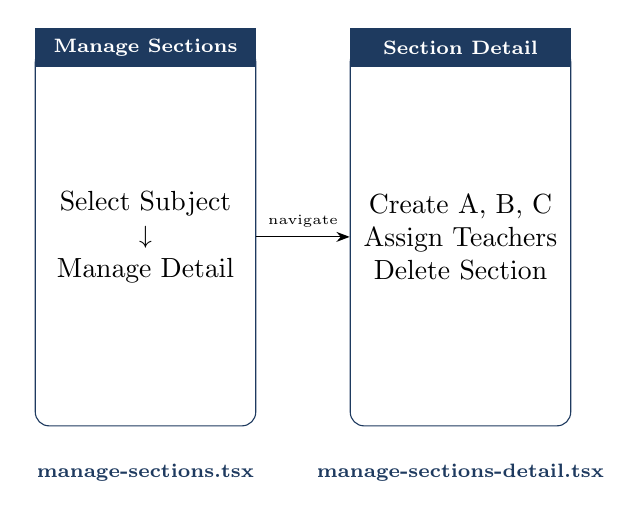
\begin{tikzpicture}[
    screen/.style={
      rectangle, rounded corners=5pt, draw=AttendPrimary, minimum width=2.8cm,
      minimum height=4.8cm, fill=white, align=center, font=\scriptsize
    },
    hdr/.style={rectangle, fill=AttendPrimary, text=white, minimum width=2.8cm,
      minimum height=0.5cm, font=\scriptsize\bfseries}
  ]
    \node[screen] (s1) at (0,0) {};
    \node[hdr] at (s1.north) {Manage Sections};
    \node[align=center] at (s1.center) {Select Subject\\\small$\downarrow$\\Manage Detail};

    \node[screen] (s2) at (4,0) {};
    \node[hdr] at (s2.north) {Section Detail};
    \node[align=center] at (s2.center) {Create A, B, C\\Assign Teachers\\Delete Section};

    \draw[-{Stealth}] (s1) -- node[above, font=\tiny]{navigate} (s2);

    \node[font=\scriptsize\bfseries, text=AttendPrimary] at (0,-3) {manage-sections.tsx};
    \node[font=\scriptsize\bfseries, text=AttendPrimary] at (4,-3) {manage-sections-detail.tsx};
  \end{tikzpicture}
  \caption{%
    \textbf{Department Admin section setup flow.}%
    Admin selects a subject, creates named sections, assigns one or more teachers per section via checkbox modal, and may delete sections. Only users with \texttt{DEPARTMENT\_ADMIN} role or above see this navigation path (Department Hub).
  }
  \label{fig:admin-flow}
\end{figure}

\textbf{Screens:}
\begin{enumerate}[leftmargin=1.5em]
  \item \texttt{manage-sections.tsx} --- Subject picker.
  \item \texttt{manage-sections-detail.tsx} --- CRUD sections + teacher assignment modal.
\end{enumerate}

\section{Teacher: Manage Section Students}

\begin{figure}[H]
  \centering
  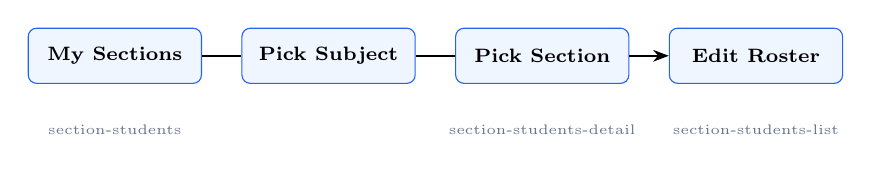
\begin{tikzpicture}[
    box/.style={
      rectangle, rounded corners=3pt, draw=AttendAccent, fill=AttendLight,
      minimum width=2.2cm, minimum height=0.7cm, align=center, font=\scriptsize\bfseries
    },
    arr/.style={-{Stealth[length=2mm]}, line width=0.6pt}
  ]
    \node[box] (a) {My Sections};
    \node[box, right=0.5cm of a] (b) {Pick Subject};
    \node[box, right=0.5cm of b] (c) {Pick Section};
    \node[box, right=0.5cm of c] (d) {Edit Roster};

    \draw[arr] (a) -- (b) -- (c) -- (d);

    \node[font=\tiny, text=AttendGray, below=0.4cm of a] {section-students};
    \node[font=\tiny, text=AttendGray, below=0.4cm of c] {section-students-detail};
    \node[font=\tiny, text=AttendGray, below=0.4cm of d] {section-students-list};
  \end{tikzpicture}
  \caption{%
    \textbf{Teacher student roster management.}%
    Teacher sees only subjects/sections from \texttt{/my-sections}. In list view they enter Edit mode, add students (filtered to exclude anyone already in another section of the same subject), or remove students. Teachers cannot create sections or assign other teachers.
  }
  \label{fig:teacher-flow}
\end{figure}

\section{Add-Student Filtering Logic}

The mobile app calls \texttt{/subjects/\{id\}/enrolled-student-ids} to build a set of students already placed in \emph{any} section of that subject. The Add Students modal only shows students \textbf{not} in that set, preventing UI attempts that would fail at the API.

% ===================== CHAPTER 6 =====================
\chapter{Integration with Attendance}
\label{ch:attendance}

\section{Attendance Session Flow}

\begin{figure}[H]
  \centering
  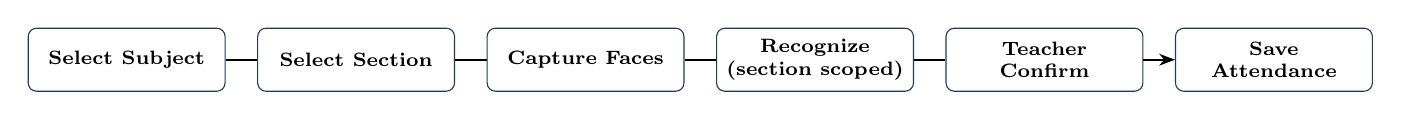
\begin{tikzpicture}[
    flowstep/.style={
      rectangle, rounded corners=3pt, draw=AttendPrimary, fill=white,
      minimum width=2.5cm, minimum height=0.8cm, align=center, font=\scriptsize\bfseries
    },
    arr/.style={-{Stealth[length=2mm]}, line width=0.6pt}
  ]
    \node[flowstep] (s1) {Select Subject};
    \node[flowstep, right=0.4cm of s1] (s2) {Select Section};
    \node[flowstep, right=0.4cm of s2] (s3) {Capture Faces};
    \node[flowstep, right=0.4cm of s3] (s4) {Recognize\\(section scoped)};
    \node[flowstep, right=0.4cm of s4] (s5) {Teacher\\Confirm};
    \node[flowstep, right=0.4cm of s5] (s6) {Save\\Attendance};

    \draw[arr] (s1) -- (s2) -- (s3) -- (s4) -- (s5) -- (s6);
  \end{tikzpicture}
  \caption{%
    \textbf{Section-scoped attendance pipeline.}%
    \texttt{attendance.tsx} loads sections from \texttt{/my-sections}. \texttt{attendance-camera.tsx} sends \texttt{section\_id} on every \texttt{/recognize} request. Only students in \texttt{section\_students} for that section can match; others are treated as unknown even if recognized at college level.
  }
  \label{fig:attendance-flow}
\end{figure}

\section{Recognition Filtering (Backend)}

In \texttt{recognize\_faces()} (\texttt{attendance.py}):

\begin{enumerate}[leftmargin=1.5em]
  \item If \texttt{section\_id} provided $\rightarrow$ load student IDs from \texttt{section\_students}.
  \item Else if \texttt{subject\_id} provided $\rightarrow$ fallback to \texttt{subject\_students}.
  \item FAISS match must be in \texttt{enrolled\_ids} set; otherwise returned as \texttt{unknown: true}.
\end{enumerate}

\section{Persisted Attendance Record}

On confirm (\texttt{POST /api/v1/attendance}):
\begin{itemize}[leftmargin=1.5em]
  \item \texttt{student\_id}, \texttt{subject\_id}, \texttt{section\_id}
  \item \texttt{attendance\_date}, \texttt{timestamp}, \texttt{confidence}
  \item Optional \texttt{face\_crop\_url} in \texttt{attendance-crops} bucket
\end{itemize}

Reports can be filtered by subject and section for administrative export (PDF/Excel).

% ===================== CHAPTER 7 =====================
\chapter{Worked Example}
\label{ch:example}

\section{Scenario}

\textbf{Department:} Computer Science \quad
\textbf{Subject:} Data Structures \quad
\textbf{Sections:} A (morning), B (afternoon)

\section{Setup Steps}

\begin{table}[H]
  \centering
  \caption{Example Setup Sequence}
  \begin{tabular}{@{}clp{7cm}@{}}
    \toprule
    \textbf{Step} & \textbf{Actor} & \textbf{Action} \\
    \midrule
    1 & Dept Admin & Create Section A and Section B under Data Structures \\
    2 & Dept Admin & Assign Teacher T1 $\rightarrow$ Section A; T2 $\rightarrow$ Section B \\
    3 & Teacher T1 & Add students S1, S2, S3 to Section A roster \\
    4 & Teacher T2 & Add students S4, S5 to Section B roster \\
    5 & Teacher T1 & Take attendance: Subject = DS, Section = A \\
    6 & System & Recognize faces; only S1--S3 eligible to match \\
    7 & Teacher T1 & Confirm matches; records saved with \texttt{section\_id = A} \\
    \bottomrule
  \end{tabular}
\end{table}

\section{Conflict Example}

If T1 attempts to add S4 (already in Section B) to Section A:
\begin{itemize}[leftmargin=1.5em]
  \item Mobile UI: S4 not shown in Add Students list (filtered by enrolled IDs).
  \item Direct API call: HTTP 400 with \texttt{conflicting\_student\_ids}.
  \item Database trigger: Exception if API check bypassed.
\end{itemize}

Resolution: Remove S4 from Section B first, then add to Section A.

% ===================== CHAPTER 8 =====================
\chapter{Operations and Edge Cases}
\label{ch:ops}

\section{Deleting a Section}

Deleting a section (\texttt{DELETE /sections/\{id\}}):
\begin{itemize}[leftmargin=1.5em]
  \item Removes all \texttt{section\_teachers} and \texttt{section\_students} rows (CASCADE).
  \item Existing attendance records retain historical \texttt{section\_id} if not cascaded (depends on FK policy).
  \item Teachers lose access via \texttt{/my-sections} immediately.
\end{itemize}

\section{Section Naming}

Names are normalized to uppercase on create. Recommended convention: single letters (A, B, C) or short codes (A1, LAB1).

\section{Super Admin / Platform Admin}

Super admins with a \texttt{college\_id} may perform all dept-admin section operations for their college. Platform admins have global manage rights via \texttt{\_can\_manage\_section}.

\section{Known Limitations}

\begin{itemize}[leftmargin=1.5em]
  \item No bulk import of section rosters (manual assign via mobile UI).
  \item No automatic section assignment at student enrollment time (separate workflow).
  \item Teacher must be explicitly assigned to section before taking attendance for it.
  \item Section list for attendance comes from \texttt{/my-sections}, not all sections of subject.
\end{itemize}

\chapter{Summary}
\label{ch:summary}

Section management in Attend provides:
\begin{itemize}[leftmargin=1.5em]
  \item Structured batch organization under subjects
  \item Teacher and student assignment with strict one-section-per-subject rule
  \item Role-based administration and teacher self-service rosters
  \item Section-scoped face recognition and attendance persistence
  \item Database-level integrity via triggers and RLS
\end{itemize}

This module is implemented in \texttt{apps/backend/app/api/v1/sections.py}, migrations \texttt{001} and \texttt{002}, and mobile screens under \texttt{manage-sections*} and \texttt{section-students*}.

\end{document}
